\documentclass[a4paper,11pt,twoside,openright]{report}

\usepackage{graphicx}
%\usepackage{ngerman}
\usepackage[utf8x]{inputenc}
\usepackage{fancyvrb}
\usepackage{courier}
\usepackage{helvet}
\usepackage{tikz}
\usepackage{xcolor}
\usepackage{pdfpages}
\usepackage[strict]{changepage}
\usepackage{verbatim}

\pdfoptionpdfminorversion=6

% \definecolor{se_dark_blue}{RGB}{0,103,166} % powerpoint
\definecolor{se_dark_blue}{RGB}{0,96,178} % website
% \definecolor{se_light_blue}{RGB}{119,158,201} % powerpoint
\definecolor{se_light_blue}{RGB}{129,160,225} % website


%% setup listings
\usepackage{listings}
\lstset{
    numbers=left,
    numberstyle=\tiny,
    numbersep=5pt,
    xleftmargin=11pt,
    xrightmargin=4pt,
    frame=single,
    aboveskip=0pt,
    belowskip=-6pt,
    sensitive=true,
    float=!t,
    breaklines=false,
    captionpos=b,
    tabsize=2,
    showstringspaces=false,
    basicstyle=\small\ttfamily,
    morecomment=[l]{//},
    morecomment=[s][\itshape]{/**}{*/}
}

%% defines the listings laguage named 'MontiArc' derived from the language 'Java' 
%% adding the below listed keywords. See 
%% ftp://ftp.tex.ac.uk/tex-archive/macros/latex/contrib/listings/listings.pdf
%% for listings documentation
\lstdefinelanguage{MontiArc}[]{Java}{
  morekeywords={component, port, in, out, inv, package, import, connect, autoconnect}
}

% Seite einrichten
\setlength{\voffset}{-1in}
\setlength{\hoffset}{-1in}

\setlength{\topmargin}{2.5cm}		   
\setlength{\headheight}{0cm}		   
\setlength{\headsep}{0cm}		   
\setlength{\oddsidemargin}{3,3cm}  % innen ein wenig mehr Rand für die Klebebindung
\setlength{\evensidemargin}{2,7cm} % dafür außen ein wenig weniger
\setlength{\textwidth}{15cm}		   
\setlength{\textheight}{23,5cm}		   
\setlength{\parindent}{0cm}

\newcommand{\emptyLine}{{\LARGE ~\\}}

\begin{document}

% Einrücken von Absätzen verhindern und 1.5 Zeilen Absatzabstand
\setlength{\parindent}{0pt}
\setlength{\parskip}{1.5ex plus0.5ex minus0.5ex}

%% Dieses Teildokument beschreibt die Titelseite.
%

% Seitenzähler auf 1, Römische Ziffern.
\setcounter{page}{1}
\pagenumbering{roman}

\thispagestyle{headings}

%\changepage{<text height>}{<text width>}{<even-side margin>}{<odd-side margin>}{<column sep.>}{<topmargin>}{<headheight>}{<headsep>}{<footskip>}
\changepage{5,1cm}{2.4cm}{}{-0.7cm}{}{-2,3cm}{}{}{}

% Eigentliche Titelseite.
\begin{titlepage}
	
\begin{figure}\raggedleft
\includegraphics[height=3.0cm]{src/pic/logo.jpg}\end{figure}
  
\begin{tikzpicture}[overlay]

% horizontal lines
\draw[color=se_dark_blue, thick] (-1.6, 0.9) -- (17.4, 0.9);
\draw[color=se_light_blue, thick] (-1.4, 0.7) -- (17.4, 0.7);

% vertical lines
\draw[color=se_dark_blue, thick] (-1, 0.9) -- (-1, -24.5);
\draw[color=se_light_blue, thick] (-0.8, 0.7) -- (-0.8, -24.5);

\end{tikzpicture}

\vspace*{-1.5em}

\begin{flushleft}
  {\fontfamily{phv}  
  	{\LARGE
      Rheinisch Westfälische Technische Hochschule Aachen \\
      Lehrstuhl für Software Engineering \\}
    \vspace{3em}
  
    {\LARGE \textbf{Erste Titel-Zeile}\\} 
    {\LARGE \textbf{Zweite Titel-Zeile}\\} 
    {\LARGE \textbf{Dritte Titel-Zeile}\\} % Oder \emptyLine falls nicht Titel kürzer
    {\LARGE \textbf{Vierte Titel-Zeile}\\} % Oder \emptyLine falls nicht Titel kürzer
    \vspace{3em}
		
    {\Large \textbf{Diplomarbeit/Masterarbeit/Studienarbeit}\\}
		\vspace{3em} 
		
		{\large von\\} % presented by
    
    {\LARGE \textbf{Name, Vorname}\\}
    \vspace{3em} 
		    
    {\Large \textbf{1. Prüfer: Prof.\ Dr.\ B.\ Rumpe}\\}
    \vspace{1em} 
    {\Large \textbf{2. Prüfer: }\\}
    \vspace{1em} 
    {\Large \textbf{Betreuer: }\\}
    \vspace{7em} 

    {\large Diese Arbeit wurde vorgelegt am Lehrstuhl für Software Engineering \\}
    \vspace{1em}
    % The present work was submitted to the chair of software engineering
		{\large	Aachen, den \today\\}
  }
\end{flushleft}

\end{titlepage}

\changepage{-5,1cm}{-2.4cm}{}{0.7cm}{}{2,3cm}{}{}{}





%Dieses Teildokument beschreibt die Titelseite.
%

% Seitenzähler auf 1, Römische Ziffern.
\setcounter{page}{1}
\pagenumbering{roman}

\thispagestyle{headings}

%\changepage{<text height>}{<text width>}{<even-side margin>}{<odd-side margin>}{<column sep.>}{<topmargin>}{<headheight>}{<headsep>}{<footskip>}
\changepage{5,1cm}{2.4cm}{}{-0.7cm}{}{-2,3cm}{}{}{}

% Eigentliche Titelseite.
\begin{titlepage}
	
\begin{figure}\raggedleft
\includegraphics[height=3.0cm]{src/pic/logo.jpg}\end{figure}
  
\begin{tikzpicture}[overlay]

% horizontal lines
\draw[color=se_dark_blue, thick] (-1.6, 0.9) -- (17.4, 0.9);
\draw[color=se_light_blue, thick] (-1.4, 0.7) -- (17.4, 0.7);

% vertical lines
\draw[color=se_dark_blue, thick] (-1, 0.9) -- (-1, -24.5);
\draw[color=se_light_blue, thick] (-0.8, 0.7) -- (-0.8, -24.5);

\end{tikzpicture}

\vspace*{-1.5em}

\begin{flushleft}
  {\fontfamily{phv}  
  	{\LARGE
      RWTH Aachen University \\
      Software Engineering Group \\}
    \vspace{3em}
  
    {\LARGE \textbf{Spike\ Train\ Analysis\ in\ Mechanically}\\} 
    {\LARGE \textbf{Stimulated\ Rat\ Neural\ Fibers:}\\} 
    {\LARGE \textbf{Use\ Case\ for\ Design\ of\ OpenMNGlab\ Software}\\} % Replace with \emptyLine if title is shorter
    %{\LARGE \textbf{Forth line of title}\\} % Replace with \emptyLine if title is shorter
    \vspace{3em}
		
    {\Large \textbf{Bachelor Thesis}\\}
		\vspace{3em} 
		
		{\large presented by\\} 
    
    {\LARGE \textbf{Tartsch, Alexander Manuel}\\}
    \vspace{3em} 
		    
    {\Large \textbf{1st Examiner: Prof.\ Dr.\ rer.\ nat.\ A.\ Morrison}\\}
    \vspace{1em} 
    {\Large \textbf{2nd Examiner: apl.\ Prof.\ Dr.\ med.\ B.\ Namer}\\}
    \vspace{1em} 
    {\Large \textbf{Advisor: Dr.\ rer.\ medic.\ E.\ Kutafina}\\}
    \vspace{1em} 
    {\Large \textbf{Advisor: M.\ Sc.\ A.\ Pérez\ Garriga}\\}
    \vspace{7em} 

    {\large The present work was submitted to the Chair of Software Engineering \\}
    \vspace{1em}
    % The present work was submitted to the chair of software engineering
		{\large	Aachen, \today\\}
  }
\end{flushleft}

\end{titlepage}

\changepage{-5,1cm}{-2.4cm}{}{0.7cm}{}{2,3cm}{}{}{}




 % English cover

\clearpage

% Erklaerung

%\includepdf[pages={1},offset=-1in -1in]{Formular_Eidesstattliche_Versicherung_neu.pdf}
%\includepdf[pages={1},offset=-1in -1in]{Statutory_Declaration_in_Lieu_of_an_Oath.pdf} % English 

%\clearpage

\vspace*{2cm}
% Abstract
{\bf\Large Kurzfassung} \\ [1em] 
Eine kurze Zusammenfassung der Arbeit.

\vspace{10ex}
{\bf\Large Abstract} \\ [1em]
A short abstract of this thesis.

\cleardoublepage


\tableofcontents

\clearpage

% Ab erstem Kapitel Seiten arabisch zählen
\setcounter{page}{1}
\pagenumbering{arabic}

%\chapter{Introduction}
\begin{comment}
In this chapter I will give an introduction to the topic. I will give background information about neuropathic pain and the big picture goal of research in this field. \\
-quickly explain how the transmission of pain functions inside our bodies\\
-what is my bachelor thesis based on (paper from Roberto)\\
-contextualize thesis topic within the big picture \\
-talk quickly about openMNGlab and goal of adding analysis functionality and discuss software engineering goals for the framework\\

nociception/pain\\
neuropathic pain -> constant firing\\
measuring data -> microneurography\\
analyzing data -> openMNGlab\\
results -> ideas for problemsolving

C fibers
when these fibers fire all the time this is called neuropathic pain
\end{comment}
\section{Pain and Nociception}
%This section describes the general concept of nociception and pain.\\
%Nociception is what happens when we experience noxious stimuli. Pain is what our brain interprets these stimuli as.
An important field of study in the medical sciences is the study of pain. The IASP defines pain as "an unpleasant sensory and emotional experience associated with, or resembling that associated with, actual or potential tissue damage". The IASP is the international association for the study of pain. It is the leading global organization supporting the study and practice of pain and pain relief~\cite{iasp_2022}. \\
It is important to distinguish pain from the neurally coded response to potentially harmful stimuli, which is called nociception. The definition of pain includes the internal experience, as well as the concrete stimulus response.\\
As a result of a lesion or disease of the somatosensory nervous system people can also experience chronic neuropathic pain. Studies suggest, that around 6-10\% of people in the general population suffer from neuropathic pain~\cite{bouhassira_prevalence_2008}~\cite{van_hecke_neuropathic_2014}. Treatments for this are limited and often have side effects, which makes this disease difficult to deal with~\cite{brooks2017treatments}.\\
In order to study this further we need to understand the basic principles of how physical stimuli are transmitted and lead to potential pain in the brain.

\section{Neural Signalling}
After a stimulus is received by a corresponding receptor, the information needs to be passed to the brain.
The way that signals are transmitted from sensory input to the brain is via electrical signals inside of nerve fibers. Because signals have to travel aver a longer distance in the human body, the information is coded not in a continuous signal but through discrete events called action potentials or spikes~\cite{rieke1999spikes}~\cite{spikeGeneral}.\\
Spikes are an all or nothing event, which means that the concrete spike shape does not have an effect on the encoded message. It has been shown that information is temporally encoded via patterns and firing rates of spikes.\\
Trying to figure out how exactly information gets encoded has been a long standing research question.\\
In order to understand aspects of the neural code we want to analyze spiking patterns in C-fibers evoked by a mechanical stimulus. This might give us small hints about the encoding of information within the neural network. \\
One method to record such data is called microneurography (MNG). It is an electrophysiological technique that can measure peripheral nerve activity in awake human subjects~\cite{namer2009translational}. A needle electrode is inserted into a peripheral nerve and records its responses to stimuli. With this we only look at spikes from a single neuron, however, in reality signals are passed and processed by large quantities of neuronal clusters and what we are looking at is only a small part of encoding information~\cite{spikeGeneral}.\\
In this thesis we take a look at MNG data from Roberto de Col and try to replicate some of his analysis~\cite{roberto} using the software framework openMNGlab~\cite{schlebusch_openmnglab_2021}. While doing this take a closer look at how this particular use case is handled by the software and where it can be improved.

\section{Results}
I tested importing experimental files into openMNGlab and added some analysis code. In the end I managed to import 22 files, although with some difficulties and patchwork code. These problems lead me to propose some improvements for the software. Apart from the import of the 22 files I also added some analysis code and included the results of the analysis of one of the files in detail in this thesis.\\
I replicated some of the analysis methods used in~\cite{roberto} and concluded with the same results. We found that increased spiking activity of a nerve fiber, here evoked through electrical stimulation, leads to decreased response to a mechanical stimulus. In addition I also tried some other quantification approaches for the spike train data and added visualizations for the sample analysis.

% Die Logos sind veraltet und duerfen zurzeit nicht verwendet werden!
% Auf Seite \pageref{Logo} in Abbildung \ref{Logo} befindet sich das SE Logo.
\begin{comment}
-Neuropathic pain as basis \\
-comes with many diseases \\ 

-pain as electric signals \\
-goal to understand the firing patterns in nerve fibers \\
-microneurography as recording technique \\
-needle in vitro in patients \\
-action potentials as spikes \\
-animal data \\
-does not need fiber separation  

-OpenMNGlab \\
-currently only good for loading the data \\
-want to add analysis capabilities \\
-compute quantifiers for spike trains and recordings \\
-discuss results 
 
Software: \\
-working on jupyter notebook \\
-automate the spike analysis process \\
-integrate analysis into openMNGlab \\
-get requirements for spike analysis software 


There are many unsolved problems in the medical sciences. The one connected to this bachelor thesis is the issue of neuropathic pain.
This is a type of chronic pain that can appear at any moment without any obvious factors coming from the outside. It can stem from diseases that effect the nerves, but also from infection or injury.\\
%-TODO find number of people in Germany that suffer from neuropathic pain\\
%-TODO: Find out more details on neuropathic pain \\
Pain is transmitted as electric signals through the nerves inside our bodies. Because of this fact in order to understand different types of pain such as neuropathic pain we need to understand the transmission of electrical signals in nerve fibers.\\
Quantifying pain can be done by measuring the electrical activity of corresponding nerve fibers. By doing this we get data about the amount of electrical activity. We can also gather specifics about the way the electrical signals are being sent through the body. \\
We analyze data containing bursts of action potential activity as a potential proxy for neuropathic pain as the end goal. We do this in order to potentially detect this type of pain activity in neuropathic pain patients in the future.\\
There are multiple ways in which one can measure electrical activity in human bodies. One of these methods is called microneurography, which is the technique most relevant for the rest of this thesis.
This technique is used to record nerve activity in peripheral nerves. With this technique typically a needle gets inserted into a nerve fiber which then detects the electrical current in the fiber. Additionally, we can stimulate the nerve fiber to get certain responses. \\
Nerve fibers transmit data with the use of action potentials, short AP or spike. It has been shown in previous research that information is not transmitted by the shape or amplitude of the spikes, but the frequency and timings(reference). \\

%\section{Action potentials}
Action potentials, also called spikes, are ...\\
It has been shown that coding of information is done in the pattern of spikes. It does not matter how exactly a spike looks, spikes are treated as the same objects. 


Another aspect of this thesis is the use of a software framework for microneurography analysis. It is called OpenMNGlab and is being developed at the chair of medical informatics at the Uniklinik Aachen~\cite{schlebusch_openmnglab_2021}. Currently this framework has the capabilities to import data from different data acquisition tools, but is lacking more in depth analysis functionality. I am working on quantifying experimental data and with the help of OpenMNGlab and developing analysis functionalities, that could be integrated into OpenMNGlab in the future.

\end{comment}




\cleardoublepage


%\chapter{Data}

Because human nerve data is hard to obtain, we can also use animal data instead as a proxy. Animal data is usable as proxy because we can observe the nerve fibers in vitro but can better separate one single nerve fiber from others. In human data an additional step of fiber separation is necessary to differentiate between individual fibers. We can use the same experimental protocols on Animals as we would on humans. This way we can understand firing patterns of spikes and quantify them. The results can then be applied to human data. \\
In the case of this thesis, we are using the data from wistar rats. The data was recorded from 2011 to 2012 by Roberto de Col and was published in a paper (put reference). The goal of the paper was to evaluate the effects of spiking activity on the response to mechanical stimulation. 

-How much of the exact experimental details are supposed to go here as far as methodology goes, since this is a computer science thesis 

The experiments were done in vitro on peripheral nerve fibers. The fibers were mechanically and electrically stimulated via a custom made electromechanostimulator. The nerve activity was recorded using an electrode. The electrical stimulation consists of small electrical pulses that come in a controlled frequency. The mechanical force is applied in a sinusoidal shape. \\
For single recordings the mechanical force that is applied throughout stays at approximately the same level for most of the files (put for how many files this is the case), but there are exceptions where the mechanical stimulation changes in amplitude and length during one recording. 

The experimental software used for these experiments is called Spike2 and is described further in the background chapter.

\cleardoublepage


\chapter{Background}

-Available spike analysis frameworks \\
-fieldtrip \\\
-elephant \\
-Why they are not sufficient \\
-problem with the relays? maybe windows updates 

 

-openMNGlab as a solution \\
-acquisition frameworks we need to handle \\
-Current status of openMNGlab, including Neo \\
-go into detail on different data acquisition softwares \\
-Dapsys, OpenEphys, Spike2 \\
-why does dapsys not work in the future \\

  

When deciding with which software to analyze the data there were multiple possibilities. 

There are the existing FieldTrip and Elephant tools, as well as the Software framework openMNGlab,  that all offer different analysis opportunities for electrophysiology data. 

Fieldtrip (fieldtriptoolboX.org) is a software developed at the Radboud University, Nijmegen, the Netherlands and offers a wide variety of analysis functions. The main problem with this software is its programming language. It is a MATLAB toolkit, however it would be preferred to use a software package in python or another programming language that slots better in the already existing structure within the chair for medical informatics. In addition to that it is not only speficied for spike trains software, dealing with MEG, EEG and iEEG analysis. 

Elephant (https://elephant.readthedocs.io/en/latest/index.html) is a python module which offers some high-level analysis functions for spike trains specifically. The main problem with this software is the lack of basic functionalities. It relies more on highly specified analysis tools that are not necessarily viable in our use-case. For the use in this thesis I want to start with the basic signal from the spikes, try out different quantifiers and look at the data from a fresh perspective. 

In the end I decided on using the software framework openMNGlab. It is a python framework being developed at the chair of medical informatics RWTH. It offers some basic import and analysis functionalities that are ideal for using in this Bachelor thesis. With this framework I can start from the beginning and develop my own quantifiers. 


\section{Data acquisition software} 
There are many different data acquisition software packages for electrophysiological data. 

\subsection{Spike2}
“Spike2 is a multi-channel continuous data acquisition and analysis package”( https://ced.co.uk/products/spkovin) produced by Cambridge electronic design limited. \\
-Used for the experiments I am analysing by Roberto \\
-records data in multiple channels \\
-channel for raw signal \\
-channel for mechanical force \\
-channel for event markers \\
-channel for temperature (not used by me) \\
-channel for comments (used for marking when chemicals are applied) \\
-spikes can be separated into own channels (done by experimenters) \\
-software offers a graphical representation of the data \\
-channels are separated \\
-was used for confirmation of what the data should output in terms of basic quantifiers \\
-can export csv files from the data \\
-has direct importer in openMNGlab \\

Spike2 is a data acquisition and analysis software produced by Cambridge electronic design limited. It is a flexible tool that can be used in a variety of different ways.

TODO: go into detail\\

\begin{figure}
	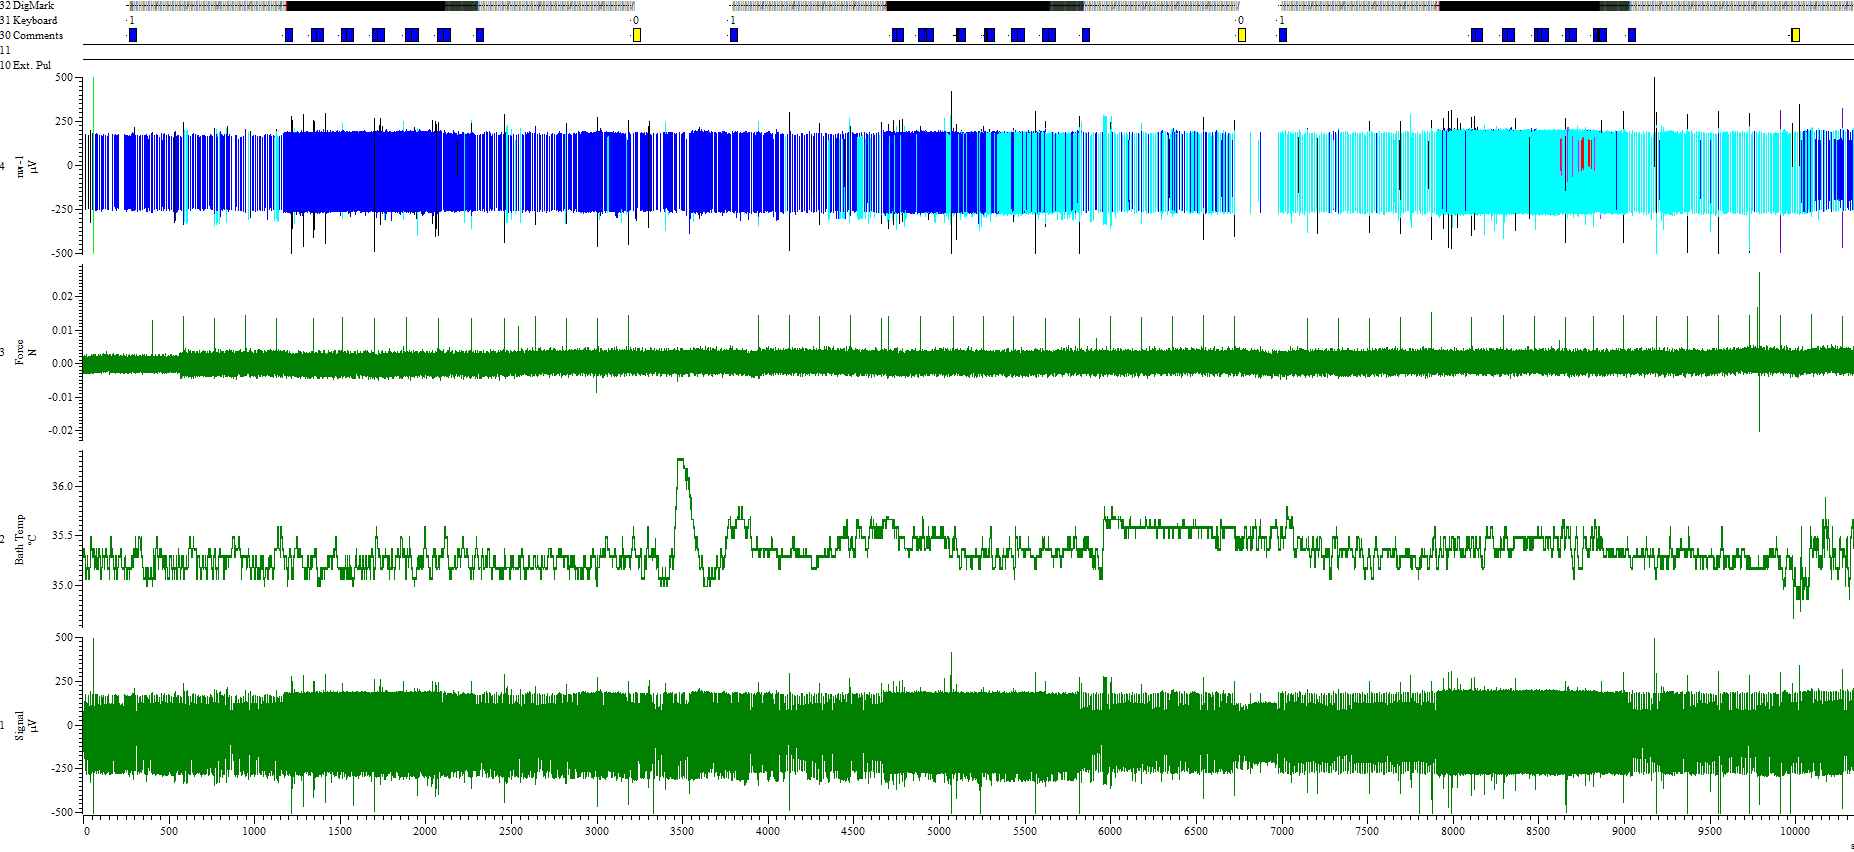
\includegraphics[width = \textwidth]{src/pic/Spike2_screenshot}
	\caption{Typical mechanically and electrically stimulated recording in Spike2}
	\label{fig:spike2}
\end{figure}

The software can record multiple channels simultaneously. An example screenshot from a recording can be seen in Figure~\ref{fig:spike2}. This depicts a typical recording used for analysis in this bachelor thesis. The recording contains data from nerve fibers of rat cranial dura mater. The nerve fibers were stimulated using a mechanoelectrostimulator applying electaical and mechanical stimulation. 

\begin{figure}
	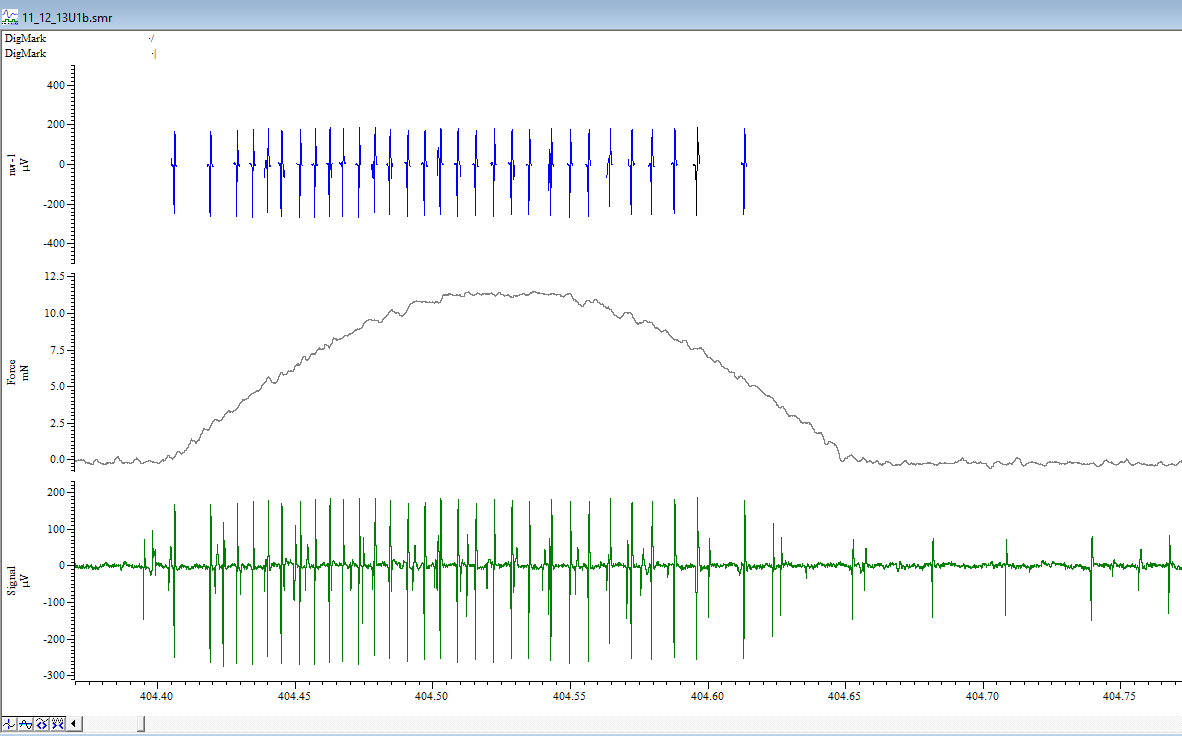
\includegraphics[width = \textwidth]{src/pic/Spike2_spike_train}
	\caption{A single spike train in spike2}
	\label{fig:spike_train}
\end{figure}

First of all it contains a channel for the recorded raw signal at the bottom. The next channel contains the temperature during the recording. In this example it fluctuates between 35°C and 36.5°C. In channel 3 we can observe the mechanical force that was applied to the nerve fibers. In Figure~\ref{fig:spike2} there are spikes in mechanical force whenever a mechanical stimulation occurs to evoke a spike train. For this experiment we want to collect the data of single nerve fibers. It is diffucult, to record just a single nerve fiber in vitro, however. This is why in this experiment spike templates are applied to the raw signal to filter out specific fibers. These filtered fibers are then displayed in channel 4, where only the action potentials of selected shapes are collected.\\
The topmost channel in Figure~\ref{fig:spike2} contains markers for the electrical and mechanical stimuli. Additionally there is a channel containing comments regarding the experiment. Comments can represent the experimental protocol and are filled in by the experimenters. In this example there are comments denoting a change electrical stimulation frequency. In other experiments for example, these could also denote the application of certain chemicals towards the recorded subject.

A more detailed view of a single spike train can be seen in Figure~\ref{fig:spike_train}. Here the difference in electrical and mechanical event markers in the topmost chanel can be seen. Mechanical markers are represented by a slash, while electrical markers are represented by a vertical line. Another thing that can be seen here is the channel containing only the spikes. This channel is ideal for the extraction of the spikes for later analysis as there is no noise in the channel anymore and the spikes can also be interpreted as simple events with a timestamp.

\subsection{Dapsys}
“DAPSYS is a combined hardware and software system designed for real-time acquisition and display of data and synchronous control of stimulators.” (http://www.dapsys.net/) \\
-Used by Barbara for her experiments \\
-used for mng-experiments with human patients \\
-also has a graphical representation of the data \\
-has importer in openMNGlab \\
-needs to export specific templates for the importer to work \\
-Dapsys has problem in the future \\
-it gets harder to set up experimental protocols \\
-maybe it has something to do with newer windows updates \\
-that means this will probably not be used much in the future \\



\subsection{OpenEphys}
OpenEphys \\
-open-source electrophysiology \\
-based in Cambridge, Massachusetts \\
-Used in experiments in Bristol cooperation \\

 
\cleardoublepage


\chapter{Software}

-Use-cases:\\
	\null\quad-opening data (importing)\\
	\null\quad-latency study (Alina)\\
	\null\quad-chemical data study (Jessica)\\
	\null\quad-mechanically evoked spike trains (Alexander)\\
	\null\quad-experimental researchers (Barbara)\\
-results in a list of requirements\\
-Use-cases lead to software engineering approach\\
-nessecary steps for my analysis\\
-how I implemented it



\begin{comment}
Alina \\
Works with spike2 data \\
Electrical data and mechanical data \\
Uses old way of importing currently (csv export from spike2) \\
Needed channels from csv export: \\
DigMark for electrical and mechanical stimulus events \\
WaveMark channel for timestamps of spikes \\
Information used: \\
Electrical stimulus events + timestamps \\
Calculate Latency for spikes (timestamps) \\
Calculate Spike Count  \\
In theory this information is available with the direct import of openMNGlab right now \\
Potential problems with direct openMNGlab importer: \\
Each template for spikes in spike2 results in separate channel in Neo structure after openMNGlab import -> needs some filtering (manual right now) \\
Electrical and mechanical events share a channel (DigMark) and somehow need to be distinguished if the recording also features mechanical stimulation \\
\end{comment}

The first user is a student who does data analysis on mechanically and electrically stimulated Spike2 data. The goal is to perform latency analysis for spikes.  The raw spike2 files feature a lot of information, not all of which is always needed. In this case, all that is required to analyse the latencies of the spikes are the timestamps of the spikes itself and the timestamps of the stimulation events. For the Spike2 software this means that we need to extract the DigMark channel which contains the event information as well as the wavemark channel which contains the information on the already presorted spikes.\\
The relevant information can be imported using the importing function of openMNGlab. 
 
\begin{comment}
Alexander \\
Works with spike2 data \\
Electrical and mechanically stimulated data \\
Uses a mixture of old and new importing currently \\
Needed channels from csv export: \\
Mechanical force channel \\
Spike channel for timestamps of spikes \\
Need channels from direct spike2 import: \\
Electrical stimulus channel \\
Information used: \\
Electrical stimulus events + timestamps \\
Mechanical stimulus events (duration, amplitude) + timestamps \\
Timestamps for spikes in spike trains \\
Potential problems with the Neo importer: \\
Each template for spikes results in separate spike channels in the Neo structure -> this means that the filtered spikes in the spike2 spike channels (e.g., nw-1…) need to be bundled together again \\
Mechanical force channel import does not work currently \\
Electrical and mechanical events share a channel (DigMark) and somehow need to be distinguished \\
After the import of the mechanical force channel, the mechanical stimuli need to be filtered as such (probably will not happen automatically by the importer) \\
\end{comment}

The second user is also a student who uses mechanically and electrically stimulated Spike2 data. His goal is to analyse spike trains resulting from mechanical stimulation. For this he needs also does not need all of the information contained in the raw Spike2 file. He needs the event information for mechanical and electrical stimuli as well as the mechanical force information for details of the mechanical stimuli. As well as the first user he also needs the information collected from the wavemark channels detailing the exact spiking patterns.

\begin{comment}
Jessica \\
Works with spike2 data \\
Chemical data \\
Uses Neo importer \\
Needed channels from import: \\
Spike channels for spike timestamps \\
Information used: \\
Intervals which are relevant for the application of chemicals \\
Spikes + timestamps inside those intervals \\
Which chemicals are applied when \\
Potential problems with openMNGlab importer: \\
The chemical protocols are not automatically importable and readable; There is a channel in spike2 for comments where this information is given in theory, however, the notation of what is given and how much varies from comment to comment, and one needs a good understanding of the chemicals and potentially experimental procedure \\
Comments channel is not being imported currently, even if the chemical notes where uniform; This means one must manually reed the comment channel in the spike2 software itself and manually choose some intervals which might be promising for observing chemically induced changes in spiking activity \\
\end{comment}
 

Which information should available after importing data? \\
Spikes + timestamps \\
Electrical stimulation + timestamps \\
Mechanical stimulation + timestamps, duration, amplitude \\
Information about application of other stimuli (chemicals, heat…) \\
For human data: temperature?  

Spike2 \\
Spike channels + some way to group them easily (e.g., in groups from spike2 templates) \\
Electrical event channel + some way to distinguish between electrical and mechanical events \\
Mechanical force channel (maybe optional) \\
Comments channel (maybe optional) \\
Temperature (optional) (probably needed for human data) \\

\begin{comment}
My steps in analysis: 

First, I used a jupyter notebook from Radomir. For this the data needed to be extracted from Spike2 directly in the Software. This export step leads to a single csv file for one recording with 5 channels: Time, Signal, Force, DigMark(stimulation events), Spikes 

Using the csv files I could extract the spike trains for each mechanical stimulation. The detection of the spike train worked as follows: The start of the spike train gets determined by the stimulation event. The length of the spike train is a previously set amount of time (in most cases 500ms). During this timeframe all spikes in the spike channel get put into a list that keeps track of the spike trains. This pretty basic detection of spike trains works well in this specific use case but has its limits when it comes to other kinds of data with other experimental protocols or just simply recordings without any protocols. Then because we do not have the exact starting points of the trains or bursting patterns this method of detection falls flat. 

This first jupyter notebook already made use of what later became openMNGlab. The import of the data was handled by the software framework. However, openMNGlab got some updates soon after which made some significant changes to how the importers work. In the new and improved framework, the importer worked on the original Spike2 files instead of the extracted csv files. This allows for more detailed representation of the data since much of the information was lost in the extraction before this update. However, with this new way of importing the data the mechanical stimulation was not able to be extracted. I still needed the information of the mechanical stimulation which was only contained in the extracted csv file. For this reason, in my analysis from here on, I used a hybrid of the old and new versions of openMNGlab until I was able to fix the new importer to also include the mechanical stimulation channel. 
\end{comment}

\cleardoublepage


%\chapter{Analysis}

In this chapter I will present the results of my analysis.\\
-I will present the results with the help of diagrams\\

-Describe the analysis that is done for each recording file we have:\\
-Show picture of a table with all the quantifiers as an axample and add the rest to the appendix\\
\begin{figure}
	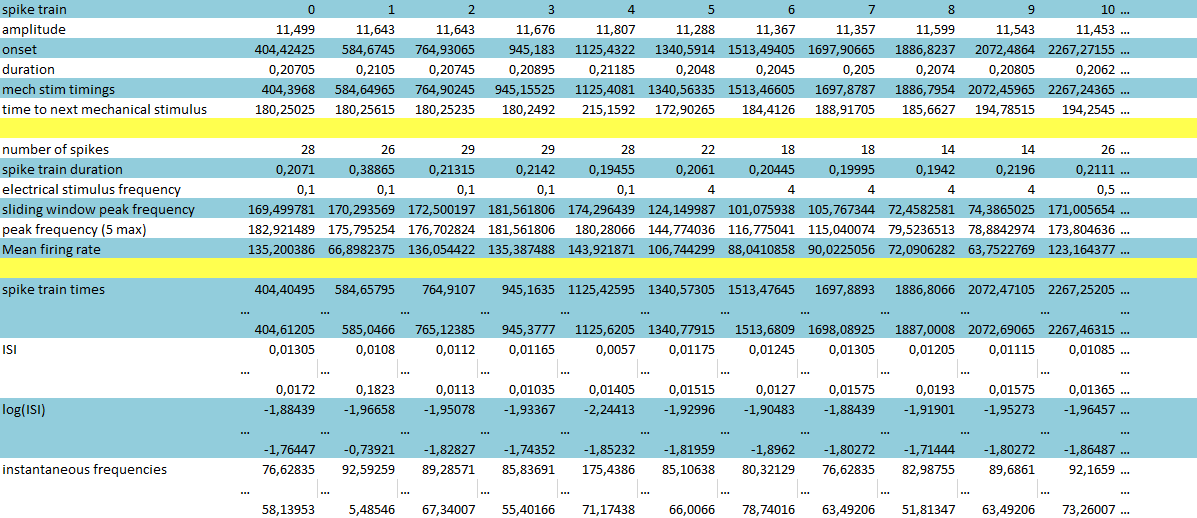
\includegraphics[width = \textwidth]{src/pic/sc_table}
	\caption{Sample picture of table after successful analysis }
	\label{fig:table_sc}
\end{figure}
-first batch contains information on the mechanical stimulus, second batch single number quantifiers about spike train, last batch lists of raw data and list quantifiers such as ISI\\
-with the help of this diagram describe the quantifiers and results that were computed\\


ausgewähltes in more detail:

-diagram of peak firing frequency, spike counts, train duration and electrical frequency\\
-shows the correlation between electrical frequency and the other quantifiers of single spike trains\\

-diagrams of Interspike Intervals(isi) and logarithm of isi\\
-should show that by taking the logarithm, the isi becomes more linear\\




\cleardoublepage


%\chapter{Code Listings}\label{ch:listings}
%% use language 'myLng' for the next listings (until another language is set)
%% include listing 'listings/AdverseReactionApp.aj' with label and caption
%% note: big listings sometimes need to overwrite the float value that has been
%% already set in the general listings setup (see paper.tex)

This chapter contains the beautiful listing \ref{lst:system}. 
Lorem ipsum dolor sit amet, consetetur sadipscing elitr, sed diam nonumy 
eirmod tempor invidunt ut labore et dolore magna aliquyam erat, sed diam 
voluptua. At vero eos et accusam et justo duo dolores et ea rebum. Stet 
clita kasd gubergren, no sea takimata sanctus est Lorem ipsum dolor sit 
amet. Lorem ipsum dolor sit amet, consetetur sadipscing elitr, sed diam 
nonumy eirmod tempor invidunt ut labore et dolore magna aliquyam erat, 
sed diam voluptua. At vero eos et accusam et justo duo dolores et ea 
rebum. Stet clita kasd gubergren, no sea takimata sanctus est Lorem 
ipsum dolor sit amet. 




\begin{figure}[hbt]
\lstset{language=MontiArc}
\lstinputlisting[
label=lst:system,
caption=Code listing with user defined syntax highlighting (MontiArc).] {src/listings/AdverseReactionApp.aj}
\end{figure}

\cleardoublepage


\chapter{Conclusion}
In this thesis spike train analysis in mechanically and electrically stimulated rat neural fibers was studied. This analysis was tested as a use case for the openMNGlab software. As a proxy for human MNG data single nerve fiber recordings from the skin nerve preparation of rats was used. The fiber was electrically stimulated to evoke different levels of spike activity, to study the effect of previous nerve fiber activity on the response to mechanical stimuli. 
The result of this was that the more the nerve fiber was active, the less was the response to mechanical stimuli. After a threshold of 2 Hz of electrical stimulation frequency the mechanically evoked spike trains contain noticeably less spikes and the peak firing frequency is significantly lower.

The openMNGlab framework was used to facilitate the analysis. The analysis of this type of mechanically stimulated data showed that the importing capabilities of the software needs improvements. Not all of the data could be loaded with the standard tools included in the framework. Other users also reported issues with the importers of openMNGlab, which is where the main work in the near future lies. The code used in this bachelor thesis can be found under \url{https://github.com/alexandertartsch/Bachelor_thesis_code/tree/v1}

% Bild einbinden
%\begin{figure}[ht!]
%\begin{center}
\includegraphics[width=5cm]{src/pic/logo}\end{center}
%\caption{Das SE Logo}
%\label{Logo}
%\end{figure}

\cleardoublepage


\bibliographystyle{alpha}
\addcontentsline{toc}{chapter}{References}
\bibliography{src/bib/Literatur}

% Begin Anhang
\appendix
\chapter{z.\,B. Programmdokumentation}

\cleardoublepage


\end{document}
